\subsection{CONTROLE DE ERRO}

\begin{comment}
In this section, we discuss about the error in analysis of the images. In this sense,
we can see that, the targets have different forms; however, 
a $ROI$ ever will have a rectangular form, so that certain areas will be more important of identify inside of $ROI$.
In Fig. \ref{fig:erroridentified}, there are some areas close of edges that target not occupies; they are
considered like error areas.

\begin{figure}[H]
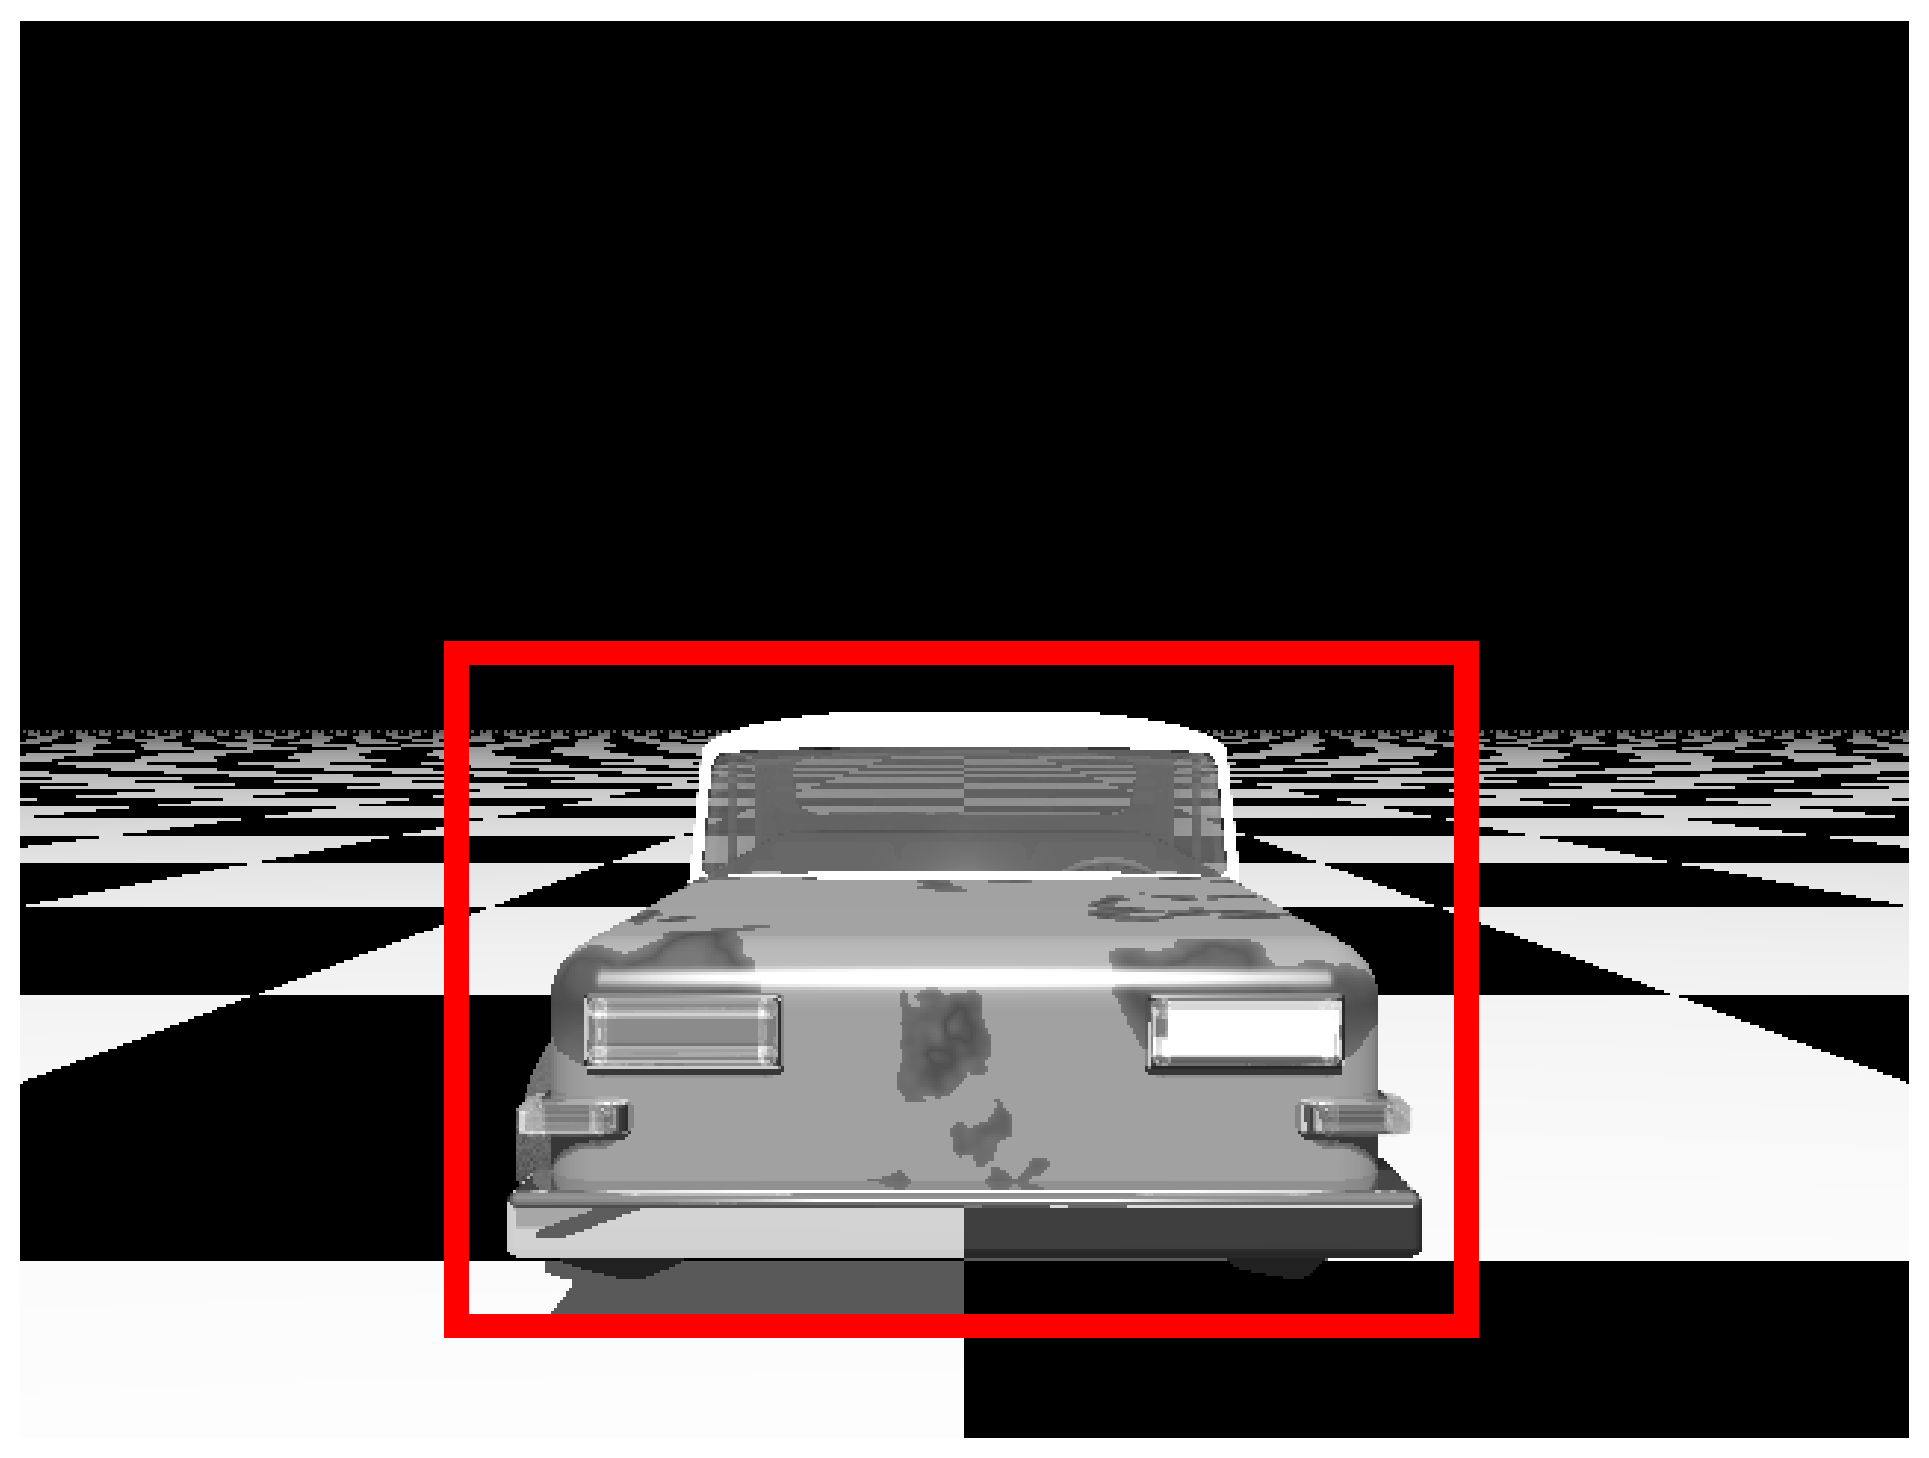
\includegraphics[width=\columnwidth]{images/imageError.eps}
\caption{Illustration of $ROI$ with error areas close of edge.}
\label{fig:erroridentified}
\end{figure}
\end{comment}

Nesta seção, é discutido o tratamento do erro produzido pela variação da forma do objeto de interesse dentro de uma
$ROI$ de forma retangular. É fácil perceber que algumas áreas próximas da borda não são ocupadas pelo objeto de interesse;
assim, elas são consideradas áreas geradoras de erro, ver Figura. \ref{fig:erroridentified}.

\begin{figure}[H]
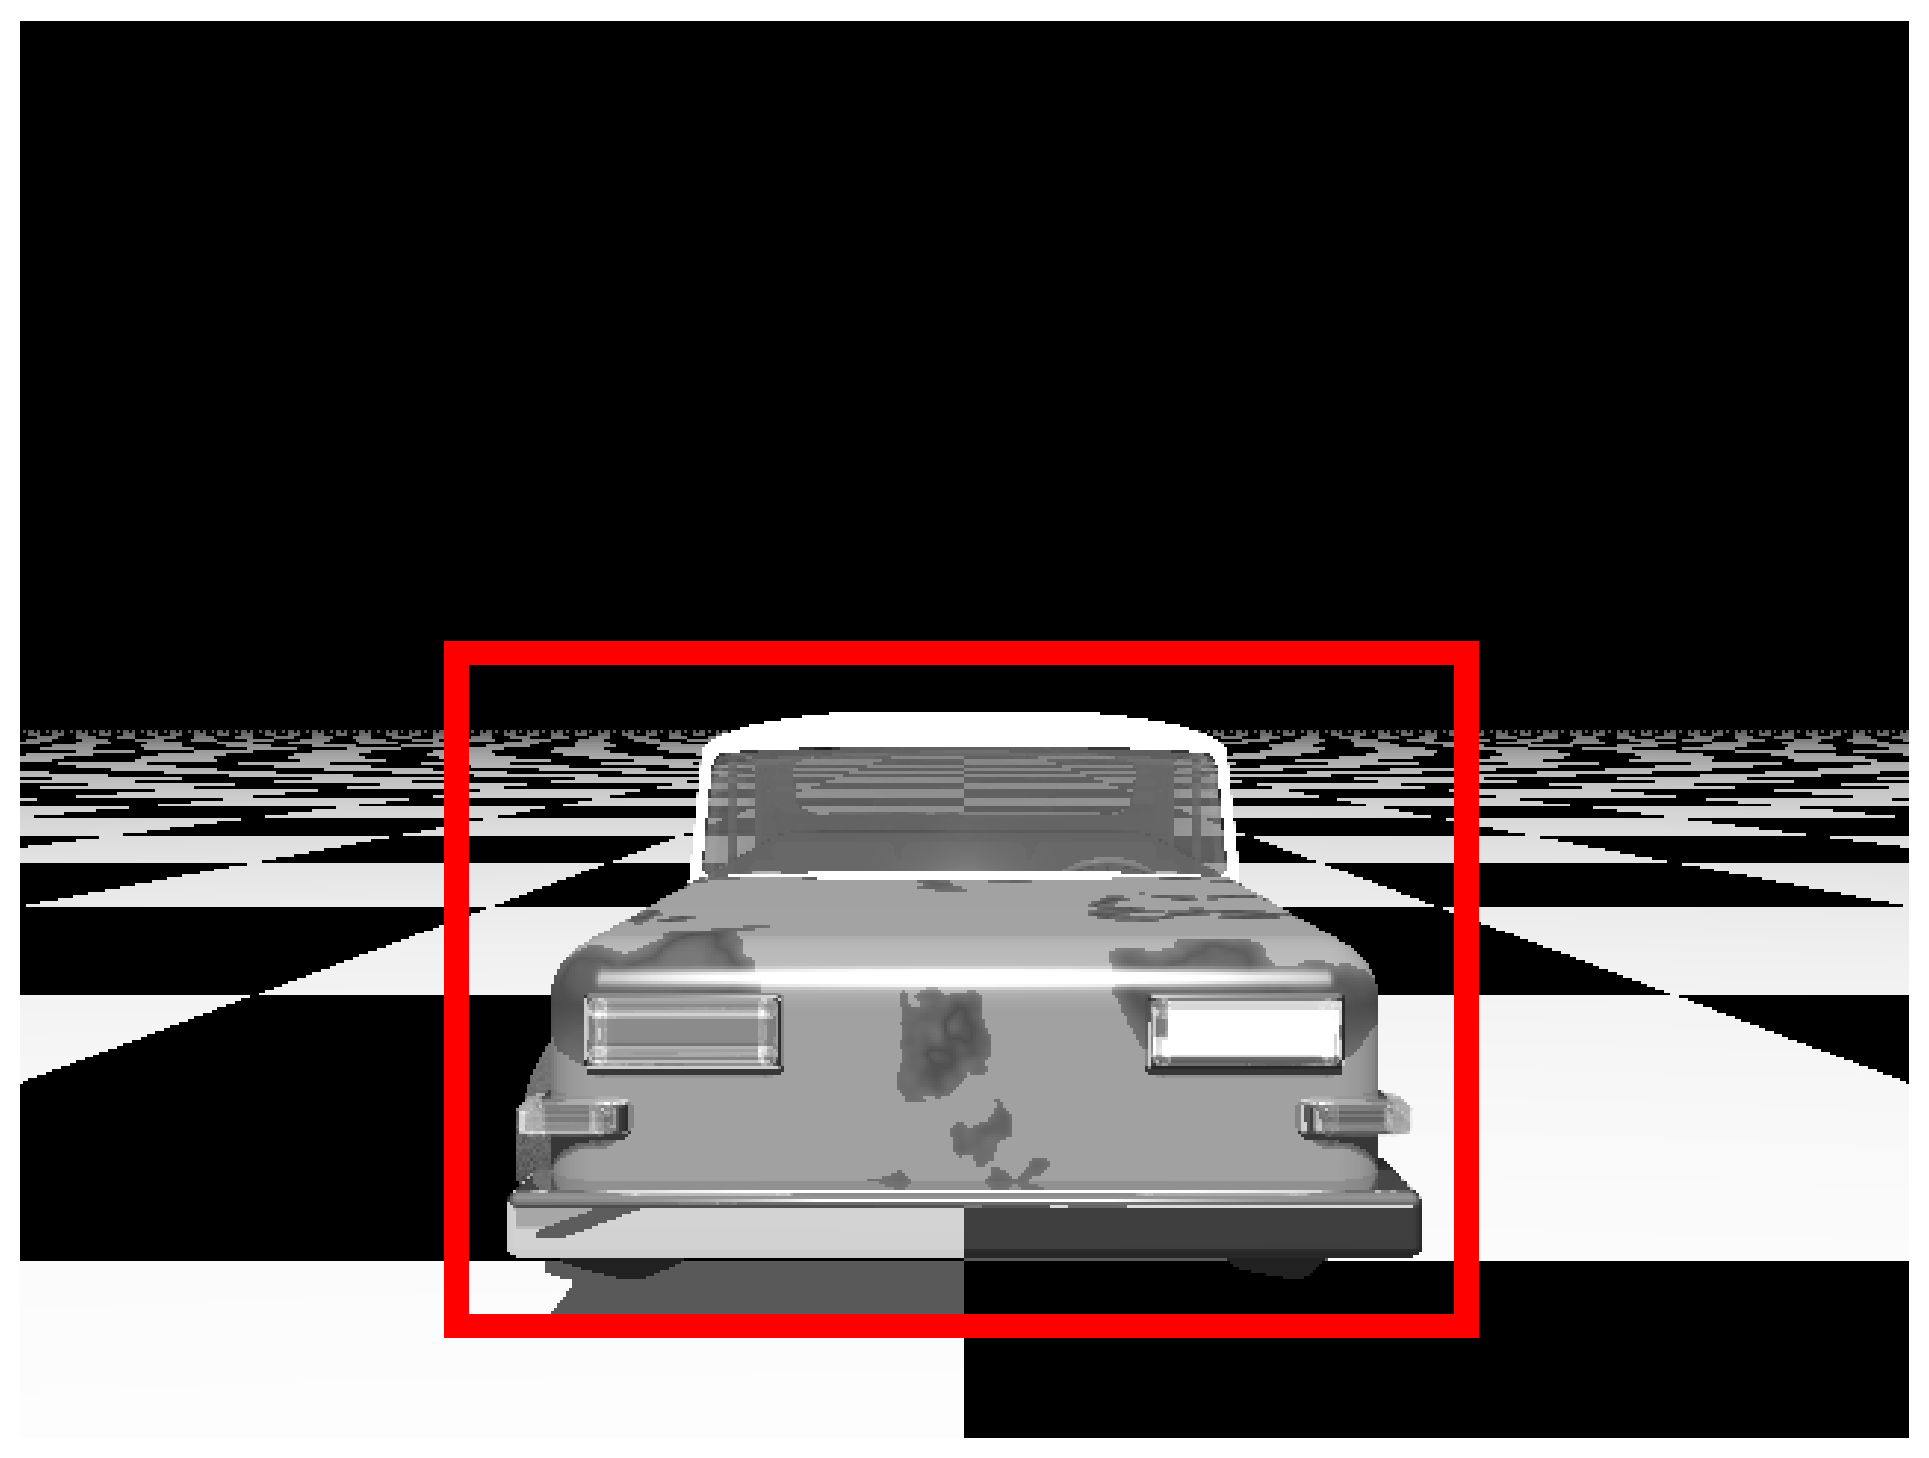
\includegraphics[width=\columnwidth]{images/imageError.eps}
\caption{Áreas geradoras de erro nas bordas da $ROI$.}
\label{fig:erroridentified}
\end{figure}

\begin{comment}
Whereas, two matrix with the same dimensions can be compared using $CCP$; 
this method of comparison doesn't generate information over the equality of the frames,
but It shows if the frames have a proportional changes for pixel values in the same position. 
Thus, if we consider a high percentage of error area when we compare the frames, It may cause 
decreasing of the correlation level between frames and will given us a fake impression that the target is out of scene.  
We decide solve this problem using a weighting matrix mask over the analyzed regions, 
before the calculus of $CCP$. This can be seen in the Fig. \ref{fig:errorpondered}.
\begin{figure}[H]
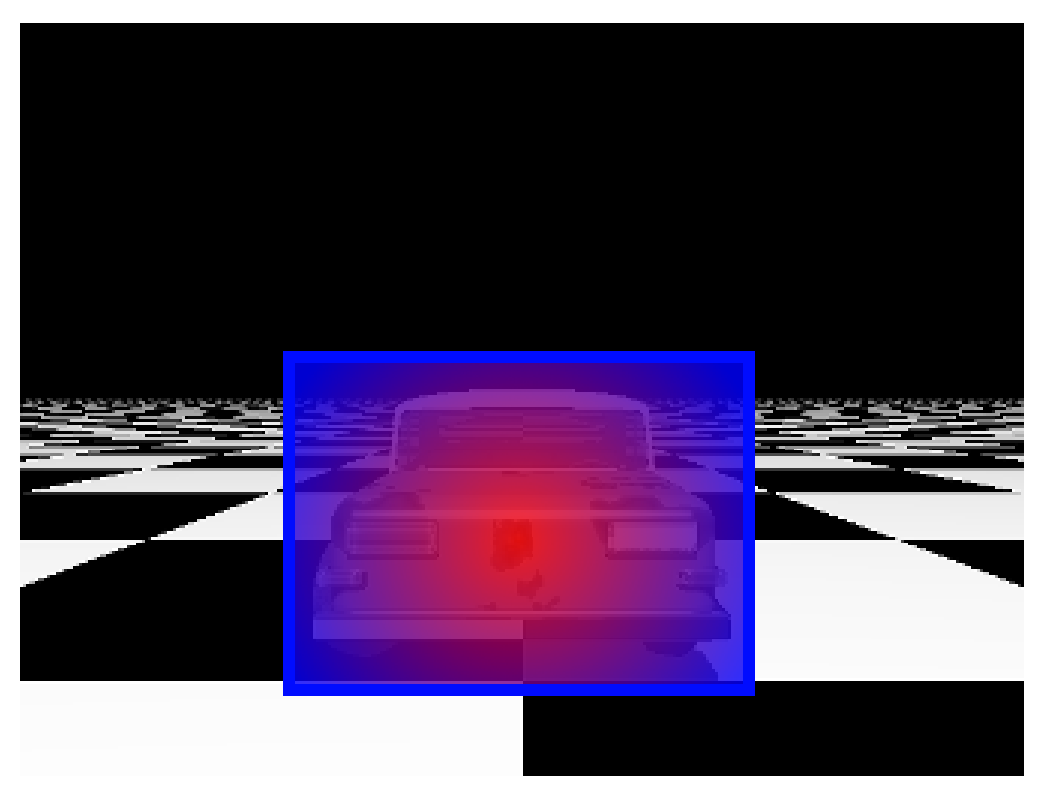
\includegraphics[width=\columnwidth]{images/imageErrorcontroled.eps}
\caption{Illustration of points of most importance (red) and points less importance (blue) in correlation.}
\label{fig:errorpondered}
\end{figure}
Where, points close of edge (in blue color) are considered of less importance, 
points close of center of image (in red color) probably are on the target, and consequently
these points are considered with more importance.
\end{comment}

O método CCP compara duas imagens (matrizes) do mesmo tamanho, 
ponderando cada $pixel$ com o mesmo peso sem importar a posição; 
consequentemente, o valor da correlação se vê reduzido visto que existem áreas produtoras 
de erro sendo usadas na comparação,
podendo assim dar uma falsa impressão de objeto perdido. 
Uma matriz de ponderação foi proposta para solucionar esse problema, como ilustrado na 
Figura \ref{fig:errorpondered}, sendo
ela é usada antes do cálculo do $CCP$.

\begin{figure}[H]
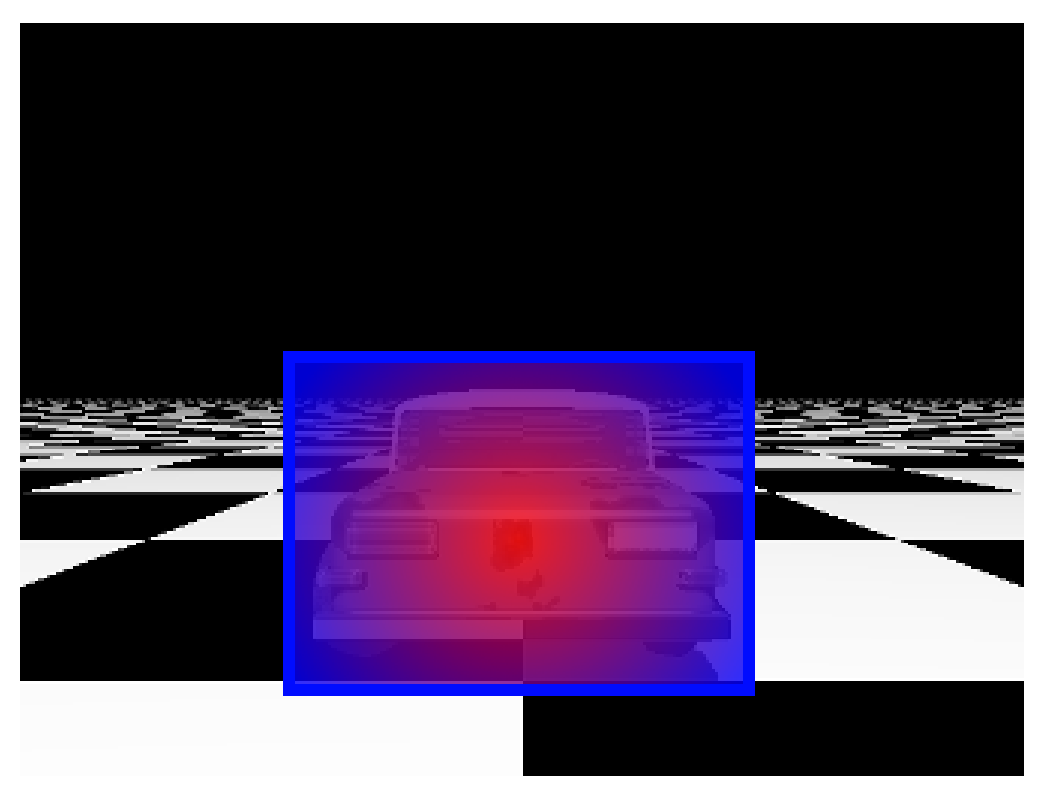
\includegraphics[width=\columnwidth]{images/imageErrorcontroled.eps}
\caption{Pontos mais significativos (vermelho) e menos significativos (azul) na correlação.}
\label{fig:errorpondered}
\end{figure}

\begin{comment}
Where, points close of edge (in blue color) are considered of less importance, 
points close of center of image (in red color) probably are on the target, and consequently
these points are considered with more importance.

Thus, to create a weighting matrix mask $Q$ like the seen in the Fig.\ref{fig:errorpondered},
we calculate the $Q(x,y)$ value as showed in the Eq. (\ref{eq:Q}), 
\begin{equation}\label{eq:Q}
 Q(x,y) = \sqrt{e^{ -\frac{|x-\mu_X|^3}{\sigma_X^3}-\frac{|y-\mu_Y|^3}{\sigma_Y^3}  }},
\end{equation}
where $Q(x,y)$ represents a value, in the line $x$ and column $y$,
$\mu_X=H/2$, $\mu_Y=W/2$, $\sigma_X=H/3$ and $\sigma_Y=W/3$; being $H$ and $W$
the height and the width, respectively, in the matrix (analysis region).

Finally, similarly to seen in the Eq. (\ref{eq:CCP}), we multiply the matrix $Q$, 
element by element, over the analysis regions
$A$ and $B$ to calculate the $r_Q$ weighted correlation coefficient, 
\begin{equation}\label{eq:rw}
 r_Q = CCP(Q~A, Q~B).
\end{equation}
\end{comment}

Os pontos próximos da borda (azul) são considerados menos importantes e os mais próximos do centro 
 (vermelho) têm maior relevância.
Assim, para criar uma matriz de ponderação $Q$, como a usada na Figura \ref{fig:errorpondered},
foi calculado $Q(x,y)$ como representado na Equação (\ref{eq:Q}),
\begin{equation}\label{eq:Q}
 Q(x,y) = \sqrt{e^{ -\frac{|x-\mu_X|^3}{\sigma_X^3}-\frac{|y-\mu_Y|^3}{\sigma_Y^3}  }};
\end{equation}
onde $Q(x,y)$ é um valor na linha $x$, coluna $y$,
$\mu_X=H/2$, $\mu_Y=W/2$, $\sigma_X=H/3$ e $\sigma_Y=W/3$; sendo $H$ e $W$
a altura e a largura, respectivamente, da região de análise.

Finalmente, pode ser usada a Equação (\ref{eq:CCP}), multiplicando a matriz $Q$ pelas 
regiões analisadas $A$ e $B$ afim de obter $r_Q$, o coeficiente ponderado de correlação de Pearson,
\begin{equation}\label{eq:rw}
 r_Q = CCP(Q~A, Q~B).
\end{equation}
